\documentclass[11pt,a4paper]{article}
\usepackage[margin=2.4cm]{geometry}
\usepackage{amsmath,amssymb,amsthm}
\usepackage{graphicx,booktabs,caption}
\usepackage[hidelinks]{hyperref}
\usepackage{microtype}
\graphicspath{{../figures/}}
\newtheorem{proposition}{Proposition}
\newcommand{\dd}{\mathrm{d}}
\newcommand{\Dt}{\Delta\tau}
\newcommand{\Dx}{\Delta x}

\title{Option Pricing Three Ways:\\[2pt]
\large Black--Scholes Formula, Finite Differences and Trinomial Trees}
\author{Aadi Mankodi\\ \small BSc Mathematics, King's College London}
\date{October 2026}

\begin{document}
\maketitle

\begin{abstract}
\noindent
A European call option is priced three ways: by the Black--Scholes formula, by
solving the Black--Scholes partial differential equation (PDE) numerically, and on a trinomial
tree. I show that the explicit finite-difference scheme and the trinomial tree are
the same algorithm. Run on the same grid, they agree to $3\times10^{-13}$. The stability limit
of the scheme is the condition that the tree's probabilities are non-negative.
The explicit scheme converges at first order and Crank--Nicolson at second order.
To reach a price error of $10^{-5}$, Crank--Nicolson is about seven times faster.
Crank--Nicolson produces a badly wrong gamma near the strike unless it is started with a few implicit
(Rannacher) steps. Finally, I price American puts, where there is no formula. The early-exercise
premium ranges from 1\% to 25\% of the European price across fifteen strikes and maturities,
and I trace the optimal exercise boundary. All code, tests and figures are in the accompanying
repository.
\end{abstract}

\section{Introduction}

The Black--Scholes model prices a European option with a formula. Most products traded in practice do not
have one: American options, barriers and options under richer models all need numerical
methods. The two standard approaches are \emph{lattice methods} (binomial and trinomial trees),
which are popular on trading desks because they are intuitive, and \emph{finite-difference
methods}, which solve the pricing PDE directly. This project builds both from scratch. I use
the closed-form price as a benchmark and measure how accurate, how fast and how robust each
method is.

The base case throughout is $S_0=K=100$, $T=1$ year, $r=5\%$ and $\sigma=20\%$. For this case the
call is worth $10.4506$ and the put $5.5735$.

\section{The model and the PDE}

\paragraph{Replication.} The share follows geometric Brownian motion,
$\dd S_t=\mu S_t\,\dd t+\sigma S_t\,\dd W_t$. Cash earns the risk-free rate $r$. Let $V(S,t)$
be the option's value. Form a portfolio that is long the option and short $\Delta$ shares. By
It\^o's formula,
\[
\dd(V-\Delta S)=\Big(V_t+\mu S V_S+\tfrac12\sigma^2S^2V_{SS}-\Delta\mu S\Big)\dd t
+\sigma S\,(V_S-\Delta)\,\dd W_t .
\]
Choosing $\Delta=V_S$ removes the random term. A riskless portfolio must earn the risk-free
rate, so $\dd(V-\Delta S)=r(V-\Delta S)\,\dd t$. This gives the \emph{Black--Scholes equation}
\begin{equation}\label{eq:bs}
V_t+\tfrac12\sigma^2S^2V_{SS}+rSV_S-rV=0,\qquad V(S,T)=\text{payoff}(S).
\end{equation}
The drift $\mu$ has disappeared: hedging removes all dependence on the share's expected return.
The companion project simulates exactly this.

\paragraph{Closed form.} For a call, \eqref{eq:bs} has the solution
$C=S\,N(d_1)-Ke^{-r(T-t)}N(d_2)$ with
$d_{1,2}=\big[\ln(S/K)+(r\pm\frac12\sigma^2)(T-t)\big]/\sigma\sqrt{T-t}$. The code
also implements the Greeks. The tests check each one against bumped prices, and check that the
Greeks satisfy \eqref{eq:bs} itself:
$\Theta+\frac12\sigma^2S^2\Gamma+rS\Delta-rV=0$ holds to $10^{-10}$. In the base case
$\Delta=0.637$, $\Gamma=0.0188$, vega $=37.5$, $\Theta=-6.41$ per year and $\rho=53.2$.

\paragraph{The log transform.} The coefficients in \eqref{eq:bs} depend on $S$, which is awkward
on a grid. With $x=\ln S$ and time to maturity $\tau=T-t$, the equation becomes
\begin{equation}\label{eq:logpde}
V_\tau=\tfrac12\sigma^2V_{xx}+\nu V_x-rV,\qquad \nu=r-\tfrac12\sigma^2,
\end{equation}
which has \emph{constant} coefficients. It is a diffusion (heat) equation with drift and
discounting, solved forward in $\tau$ from the payoff at $\tau=0$.

\section{Method 1: the explicit finite-difference scheme}

Put a uniform grid $x_j=\ln S_0+j\Dx$, $\tau_n=n\Dt$ and write $V_j^n\approx V(x_j,\tau_n)$.
Use a forward difference in $\tau$ and central differences in $x$:
\[
\frac{V_j^{n+1}-V_j^n}{\Dt}=\frac{\sigma^2}{2}\,\frac{V_{j+1}^n-2V_j^n+V_{j-1}^n}{\Dx^2}
+\nu\,\frac{V_{j+1}^n-V_{j-1}^n}{2\Dx}-rV_j^n .
\]
Rearranging gives the explicit update
\begin{equation}\label{eq:explicit}
V_j^{n+1}=p_u V_{j+1}^n+p_m V_j^n+p_d V_{j-1}^n,
\end{equation}
\[
p_u=\frac{\lambda}{2}+\frac{\nu\Dt}{2\Dx},\qquad
p_m=1-\lambda-r\Dt,\qquad
p_d=\frac{\lambda}{2}-\frac{\nu\Dt}{2\Dx},\qquad
\lambda=\frac{\sigma^2\Dt}{\Dx^2}.
\]
I fix $\lambda$ and the number of time steps $N$. Then $\Dt=T/N$ and $\Dx=\sigma\sqrt{\Dt/\lambda}$.
The spot $S_0$ is placed exactly on a node, so no interpolation is needed. The grid
extends to $\ln S_0\pm5\sigma\sqrt T$. Dirichlet boundary conditions are
$V\approx0$ (call) or $Ke^{-r\tau}-S$ (put) far below, and $S-Ke^{-r\tau}$ (call) or $0$
(put) far above.

\paragraph{Accuracy.} The local truncation error is $O(\Dt+\Dx^2)$. With $\lambda$ fixed,
$\Dx^2\propto\Dt$, so the global error should be $O(\Dt)=O(1/N)$.

\paragraph{Stability.} If $p_u,p_m,p_d\ge0$, each new value is a weighted average of old ones
with weights summing to $1-r\Dt<1$. Errors therefore cannot grow (a discrete maximum principle).
The binding condition is $p_m\ge0$, that is,
\begin{equation}\label{eq:stab}
\lambda\le 1-r\Dt\approx 1 .
\end{equation}
A von Neumann analysis gives the same answer. Substituting $V_j^n=g^n e^{ij\theta}$ gives an
amplification factor $g(\theta)=p_m+(p_u+p_d)\cos\theta+i(p_u-p_d)\sin\theta$. The
highest-frequency mode $\theta=\pi$ has $g=1-2\lambda-r\Dt$, and $|g|\le1$ again needs
$\lambda\lesssim1$. Once $\lambda>1$, the sawtooth mode $(-1)^j$ is multiplied by roughly
$2\lambda-1>1$ at every step and blows up.

\section{Method 2: the trinomial tree, which is the same thing}

A recombining trinomial tree moves the log price up by $\Dx$, leaves it unchanged, or moves it
down by $\Dx$ over each step $\Dt$, with risk-neutral probabilities $q_u,q_m,q_d$. Backward
induction gives $V=D\,(q_uV_{\text{up}}+q_mV_{\text{mid}}+q_dV_{\text{down}})$ with discount
factor $D$.

\begin{proposition}
Let $q_k=p_k/(1-r\Dt)$ for $k\in\{u,m,d\}$ and $D=1-r\Dt$. Then the tree reproduces the explicit
scheme \eqref{eq:explicit} exactly, and the $q_k$ are probabilities if and only if the
stability condition $p_k\ge0$ holds. They match the first two moments of the log-price
increment to leading order:
\[
(q_u-q_d)\Dx=\frac{\nu\Dt}{1-r\Dt},\qquad (q_u+q_d)\Dx^2=\frac{\sigma^2\Dt}{1-r\Dt}.
\]
\end{proposition}

\noindent The proof is immediate: $p_u+p_m+p_d=1-r\Dt$, and multiplying out gives
\eqref{eq:explicit}. The point is the interpretation. The PDE scheme is a random walk under the
risk-neutral measure, and \emph{a negative middle probability is exactly what makes the scheme
unstable}.

\paragraph{Why the agreement is exact.} After $N$ steps, the value at $S_0$ depends only on the
$2N+1$ nodes within $N$ steps of it. This is the scheme's domain of dependence, and it is
exactly the tree. If the grid has at least $N$ nodes on each side of $S_0$, the boundary
conditions never reach the answer. Table~\ref{tab:tree} confirms this for European calls and
American puts: the largest difference across all runs is $2.8\times10^{-13}$, which is
floating-point rounding. The more common tree discount $e^{-r\Dt}$ differs from $1-r\Dt$ by
$O(\Dt^2)$ per step, which shifts the price by $O(\Dt)$ in total. The convergence plot shows
this as a curve sitting just below the explicit scheme's.

\begin{table}[h]\centering\small
\begin{tabular}{rlccc}
\toprule
$N$ & option & explicit FD & trinomial tree & $|\text{difference}|$\\
\midrule
10   & European call & 10.376455406422 & 10.376455406422 & $4.6\times10^{-14}$\\
100  & European call & 10.443056135114 & 10.443056135114 & $8.5\times10^{-14}$\\
1000 & European call & 10.449829743431 & 10.449829743432 & $2.8\times10^{-13}$\\
10   & American put  & 6.019863420594  & 6.019863420594  & $1.2\times10^{-14}$\\
100  & American put  & 6.083551972862  & 6.083551972862  & $5.8\times10^{-14}$\\
1000 & American put  & 6.089725322509  & 6.089725322509  & $1.1\times10^{-13}$\\
\bottomrule
\end{tabular}
\caption{Explicit scheme against trinomial tree, $\lambda=0.5$, grid of half-width $N$.}
\label{tab:tree}
\end{table}

\section{Method 3: Crank--Nicolson}

The $\theta$-scheme averages the spatial operator $\mathcal L$ (the right-hand side of
\eqref{eq:logpde}) between the old and new time levels:
\[
(I-\theta\Dt\,\mathcal L_h)V^{n+1}=(I+(1-\theta)\Dt\,\mathcal L_h)V^n .
\]
Here $\theta=0$ is the explicit scheme, $\theta=1$ fully implicit, and $\theta=\tfrac12$ is
\emph{Crank--Nicolson} (CN). For $\theta>0$ each step requires solving a tridiagonal linear
system. This costs $O(J)$ operations for $J$ grid points (\texttt{scipy.linalg.solve\_banded}).
In exchange, CN is stable for \emph{any} $\Dt$ and is second-order accurate in both $\Dt$ and
$\Dx$.

Its weakness is the payoff kink at $S=K$. CN is not positivity-preserving: high-frequency modes
are damped by a factor close to $-1$ per step when $\Dt\gg\Dx^2$. A kink contains every
frequency, and the resulting oscillation is invisible in the price but ruins the second
derivative, gamma. The standard fix is \emph{Rannacher time-stepping}: replace the first CN step
or two with fully implicit half-steps, which damp the high frequencies strongly, and then switch
to CN.

\section{Results}

\subsection{Convergence and cost}

Figure~\ref{fig:conv} (left) plots the absolute pricing error against grid size. A least-squares
fit on log--log axes gives slopes of $-1.00$ for the explicit scheme (against time steps) and
$-1.99$ for Crank--Nicolson (against space steps), matching theory. For CN I used $N/4+1$ time
steps for $N$ space steps, because its stability does not tie $\Dt$ to $\Dx^2$.

The right panel shows the trade-off that matters in practice: error against CPU time. For a rough
price, with an error of $10^{-3}$ (a tenth of a cent), the two are equally fast, at about 5\,ms.
For high accuracy, CN wins clearly. It reaches a $10^{-5}$ error with 3{,}200 space steps in
about 0.1\,s. The explicit scheme needs about 75{,}000 time steps for the same error and takes
about 0.8\,s, roughly seven times longer. The reason is the stability constraint. Halving $\Dx$
forces the explicit scheme to quarter $\Dt$, so its cost grows like $N^{3/2}$.

\begin{figure}[h]\centering
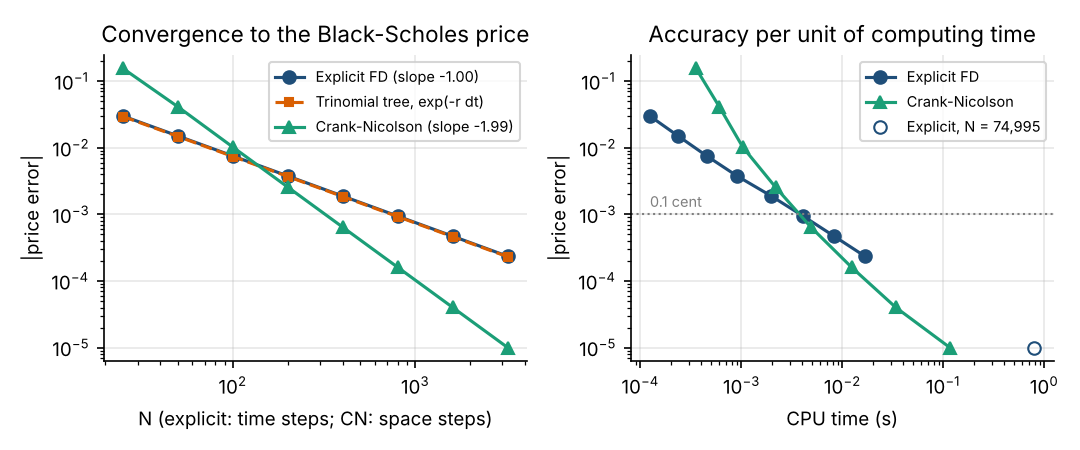
\includegraphics[width=\textwidth]{convergence.png}
\caption{Left: error against resolution, with fitted slopes. Right: error against CPU time; the
hollow point is the explicit scheme run until it matches CN's best accuracy.}
\label{fig:conv}
\end{figure}

\subsection{Stability}

Figure~\ref{fig:stab} runs the explicit scheme with 400 time steps for a range of $\lambda$.
Below $\lambda=1$ the error is small, between $1\times10^{-4}$ and $2\times10^{-3}$. It is
smallest near $\lambda\approx0.9$, where the $O(\Dt)$ and $O(\Dx^2)$ error terms have opposite
signs and partly cancel. At $\lambda=1$, $p_m=-1.25\times10^{-4}$, only just negative, and the
error is already 14 times larger than at $\lambda=0.99$. At $\lambda=1.01$ the error is 14, at $\lambda=1.02$ it is
$3\times10^4$, and at $\lambda=1.05$ it is $10^{14}$. The left panel shows the cause: the
sawtooth mode grows outward from the strike, where the payoff kink seeded it. This is the
mechanism the stability analysis predicts.

\begin{figure}[h]\centering
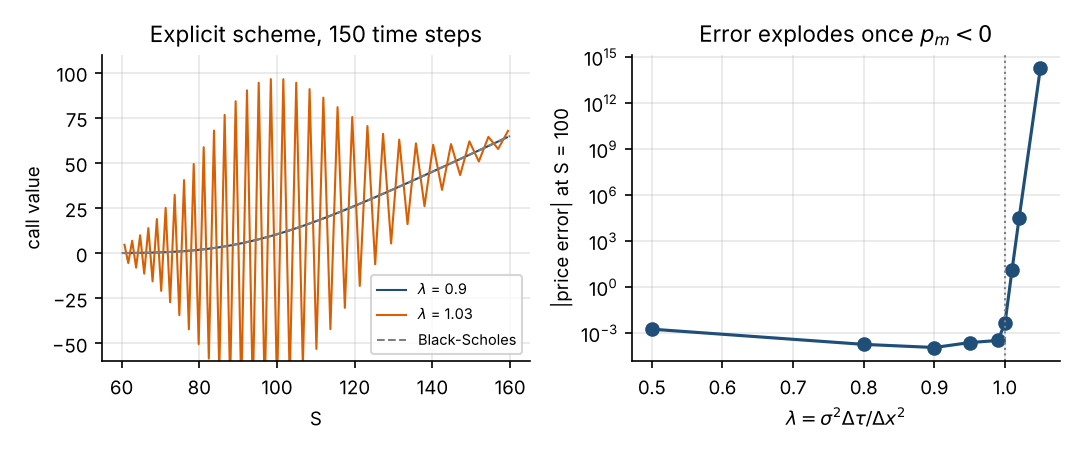
\includegraphics[width=\textwidth]{stability.png}
\caption{Left: the solution at $t=0$ with $\lambda=0.9$ (indistinguishable from Black--Scholes)
and $\lambda=1.03$ (150 steps). Right: price error against $\lambda$, 400 steps.}
\label{fig:stab}
\end{figure}

\subsection{Greeks, and why Crank--Nicolson needs Rannacher}

Greeks can be read off the grid at no extra cost. In $x=\ln S$, $\Delta=V_x/S$ and
$\Gamma=(V_{xx}-V_x)/S^2$. With 3{,}200 explicit steps the grid gives $\Delta=0.63684$ and
$\Gamma=0.018761$, against exact values of $0.63683$ and $0.018762$.

Figure~\ref{fig:gamma} uses a harsher setting: a 3-month option with only 20 CN time steps on an
800-point grid. That is efficient for the price, but plain CN produces a gamma that swings
between $-0.6$ and $1.2$ around the strike, against a true value of about $0.04$. The maximum
gamma error near the strike is $1.15$. Two Rannacher start-up steps reduce it to
$2\times10^{-5}$ at almost no extra cost. A risk system that reports gamma from a CN pricer
without this fix would show large, spurious gamma exposure around every strike.

\begin{figure}[h]\centering
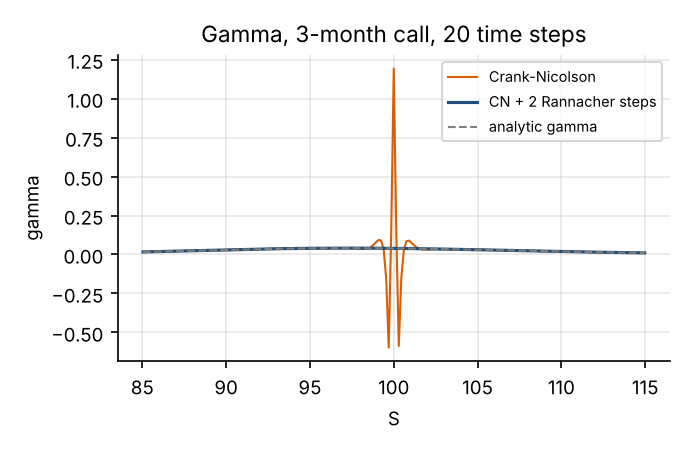
\includegraphics[width=0.62\textwidth]{gamma_rannacher.png}
\caption{Gamma of a 3-month call from Crank--Nicolson with and without Rannacher start-up.}
\label{fig:gamma}
\end{figure}

\subsection{American puts}

An American option can be exercised at any time, so its value satisfies
$V\ge\text{payoff}$ everywhere. Holding is optimal where \eqref{eq:bs} holds; elsewhere
exercising immediately is optimal. The boundary between the two regions, $S^*(t)$, is not known
in advance (a free-boundary problem), and there is no closed form. On a tree or explicit grid the fix is a single
line: after each backward step, replace $V$ by $\max(V,\text{payoff})$. This is dynamic
programming. At each node the holder compares the value of waiting with the value of exercising
now.

\paragraph{Validation.} The at-the-money one-year American put is worth 6.0901 (tree, 2{,}000
steps), against the published benchmark of 6.0904. An American \emph{call} on a non-dividend
paying share is worth exactly its European price in the code, as theory says. This is because
$C\ge S-Ke^{-r\tau}>S-K$, so exercising early is never optimal.

\begin{table}[h]\centering\small
\begin{tabular}{rrrrrr}
\toprule
$T$ & $K$ & European & American & premium & premium (\%)\\
\midrule
0.25 & 80  & 0.028 & 0.028 & 0.0003 & 1.2\\
0.25 & 100 & 3.373 & 3.480 & 0.107 & 3.2\\
0.25 & 120 & 18.709 & 20.000 & 1.291 & 6.9\\
1    & 80  & 0.687 & 0.724 & 0.036 & 5.3\\
1    & 100 & 5.574 & 6.090 & 0.517 & 9.3\\
1    & 120 & 17.395 & 20.136 & 2.741 & 15.8\\
2    & 80  & 1.507 & 1.670 & 0.163 & 10.8\\
2    & 100 & 6.611 & 7.723 & 1.112 & 16.8\\
2    & 120 & 16.509 & 20.681 & 4.173 & 25.3\\
\bottomrule
\end{tabular}
\caption{Early-exercise premium of American puts ($S_0=100$, $r=5\%$, $\sigma=20\%$).
The full grid of fifteen cases is in \texttt{results/american\_put\_premium.csv}.}
\label{tab:am}
\end{table}

Table~\ref{tab:am} shows the premium rising with both strike and maturity. Deeper
in-the-money puts and longer lives make it more valuable to receive $K$ early and earn interest
on it. The 3-month put struck at 120 is worth exactly $20.000$, its intrinsic value: it should
be exercised immediately. Figure~\ref{fig:am} shows the exercise boundary for $K=100$. Today the
put should be exercised if $S\le81.0$. The boundary rises towards the strike as expiry
approaches. The staircase shape comes from the grid spacing $\Dx$.

\begin{figure}[h]\centering
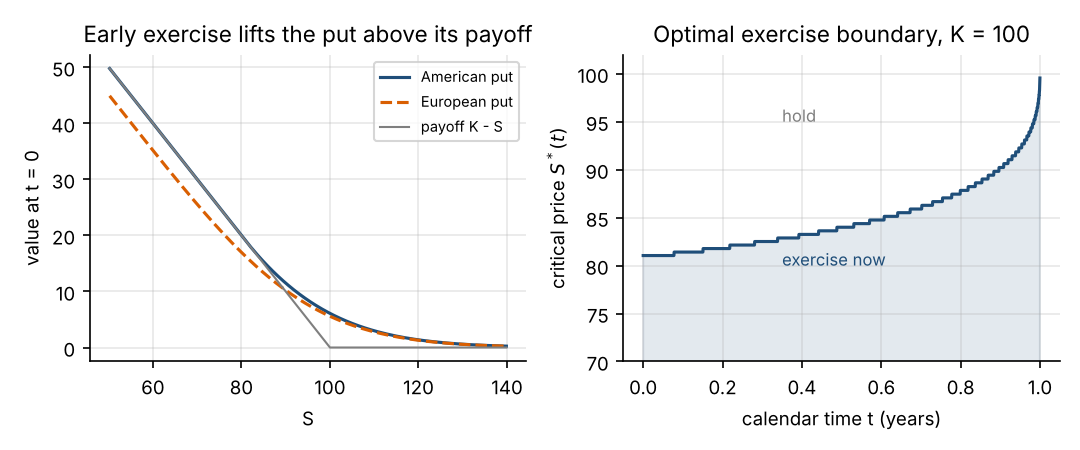
\includegraphics[width=\textwidth]{american_put.png}
\caption{Left: American and European put values at $t=0$. Right: the optimal exercise boundary
$S^*(t)$, from the explicit scheme with 4{,}000 steps.}
\label{fig:am}
\end{figure}

\section{Discussion and limitations}

\begin{itemize}
\item \textbf{Which method to use.} Trees are transparent and handle early exercise trivially, but
they are explicit schemes and inherit first-order convergence and the stability constraint.
Crank--Nicolson with Rannacher start-up is the better general-purpose tool. American options under CN need a
projected solver (PSOR or a penalty method), which I have not implemented.
\item \textbf{Strike placement.} The convergence study is at the money, where the payoff kink sits on
a grid node. For other strikes the error oscillates as the grid is refined. The usual remedies
are to align the grid with the strike or to smooth the payoff over one cell.
\item \textbf{Model.} Volatility and rates are constant and there are no dividends. Discrete
dividends would make early exercise of calls optimal in some cases, and local or stochastic
volatility would make the PDE coefficients vary. The finite-difference code extends to both
more naturally than the closed form does.
\end{itemize}

\section{Conclusion}

The three methods agree, and the reasons they agree are instructive. The explicit
finite-difference scheme for the log-price Black--Scholes PDE is a trinomial tree under the
risk-neutral measure. Its stability condition is the requirement that the tree's probabilities be
non-negative. Pushing past it destroys the solution within a few hundred steps. Crank--Nicolson
removes the constraint and converges at second order, making it several times faster at high
accuracy. It needs Rannacher smoothing to give usable Greeks. American puts carry an
early-exercise premium of up to a quarter of the European price in the cases studied.

\paragraph{Reproducing the results.} \texttt{pip install -e ".[test]"}, then \texttt{pytest}
(20 tests) and \texttt{python scripts/run\_experiments.py}. Timings are from a single CPU core
and will vary by machine; the ratios should not.

\begin{thebibliography}{9}\small
\bibitem{hull} J.\,C. Hull, \emph{Options, Futures, and Other Derivatives}, Pearson.
\bibitem{whd} P. Wilmott, S. Howison, J. Dewynne, \emph{The Mathematics of Financial Derivatives},
Cambridge University Press, 1995.
\bibitem{ran} R. Rannacher, Finite element solution of diffusion problems with irregular data,
\emph{Numerische Mathematik} 43 (1984) 309--327.
\bibitem{kcl} King's College London, \emph{Mathematical Finance I}, lecture notes, 2026--27.
\end{thebibliography}

\end{document}
